\documentclass[10pt, margin=1mm,convert={density=500,outext=.png}]{standalone}
\usepackage{cmbright}
\usepackage[OT1]{fontenc}
\usepackage{graphicx}
\usepackage{amsmath}
\usepackage{booktabs}
\usepackage[table]{xcolor}
\usepackage{colortbl}
\usepackage{braket}

\graphicspath{ {../} }

% Try out cell padding to handle fractions
% Must prefix column formatters with `S'
\usepackage{cellspace}
\setlength\cellspacetoplimit{4pt}
\setlength\cellspacebottomlimit{4pt}

\definecolor{Gray}{gray}{0.95}
\newcolumntype{a}{>{\columncolor{Gray}}c}

\renewcommand{\familydefault}{\sfdefault}

% \setlength{\tabcolsep}{12pt}

\begin{document}
\small
\begin{tabular}{ccccc}
\toprule

% &
High-fidelity system  & \multicolumn{2}{c}{Offline Phase} & Online Phase\\
% \cmidrule(lr){3-4}\cmidrule(lr){5-5}
\cmidrule(lr){1-1}\cmidrule(lr){2-3}\cmidrule(lr){4-4}

% &
\hspace{0.45in}$H(\theta)\hspace{0.43in}\ket{\psi}\hspace{0.05in}=E\hspace{0.06in}~\ket{\psi}$~
%\!\!
&
\!\!\!\!Snapshots $\psi(\theta_i)$\!\!\!\!\!\!\!\!\!\!
& Projection
& Emulation ($E \approx \widetilde E$)
\\

% Steps
% &

$
\!\!
\begin{bmatrix}
\vcenter{\hbox{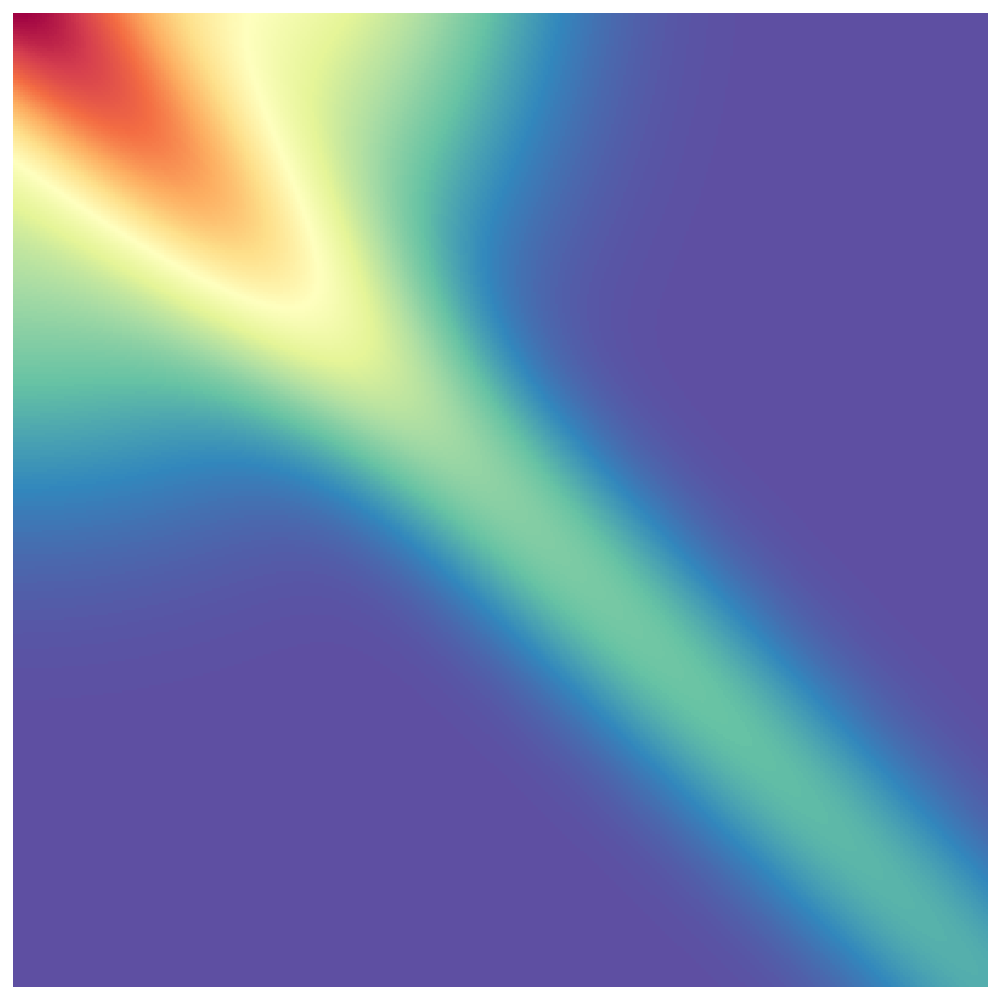
\includegraphics{highfidelity.png}}}
\end{bmatrix}
\!\!
\begin{bmatrix}
\vcenter{\hbox{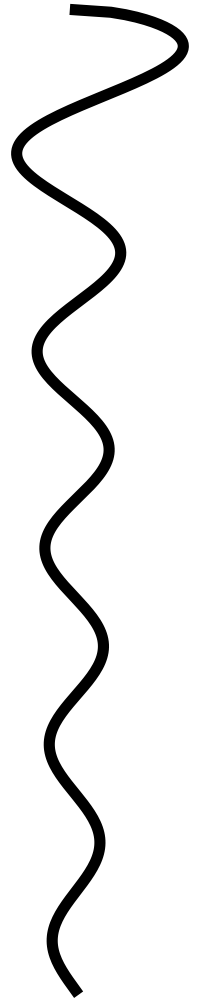
\includegraphics{wave_function.png}}}
\end{bmatrix}
\!\!
=
E
\begin{bmatrix}
\vcenter{\hbox{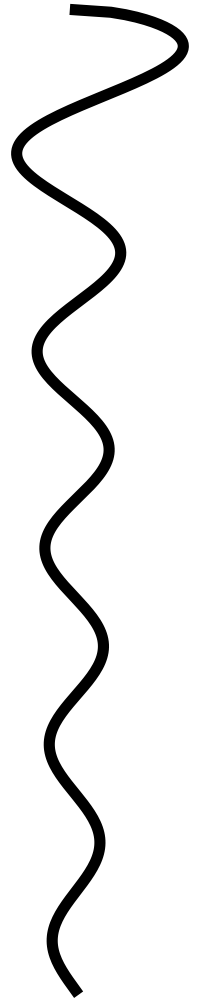
\includegraphics{wave_function.png}}}
\end{bmatrix}
%\!\!%\!\!
$

&
$
% X =
\begin{bmatrix}
\vcenter{\hbox{
\includegraphics{basis.png}}}
\end{bmatrix}
$

&

$
\!\!\!\!\!\!
\begin{bmatrix}
\vcenter{\hbox{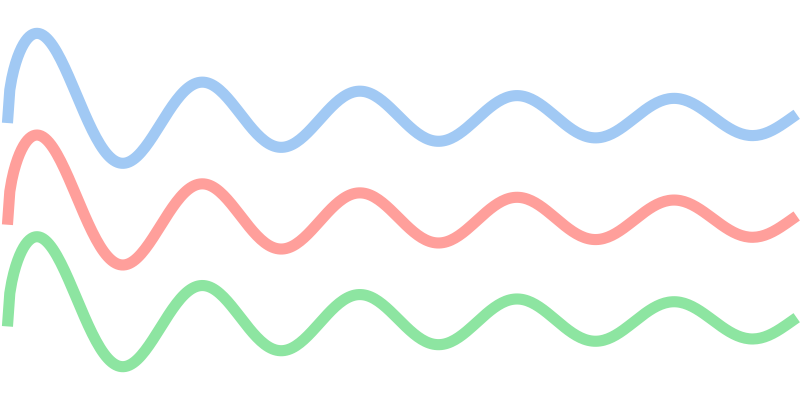
\includegraphics{basis_t.png}}}
\end{bmatrix}
\!\!
\begin{bmatrix}
\vcenter{\hbox{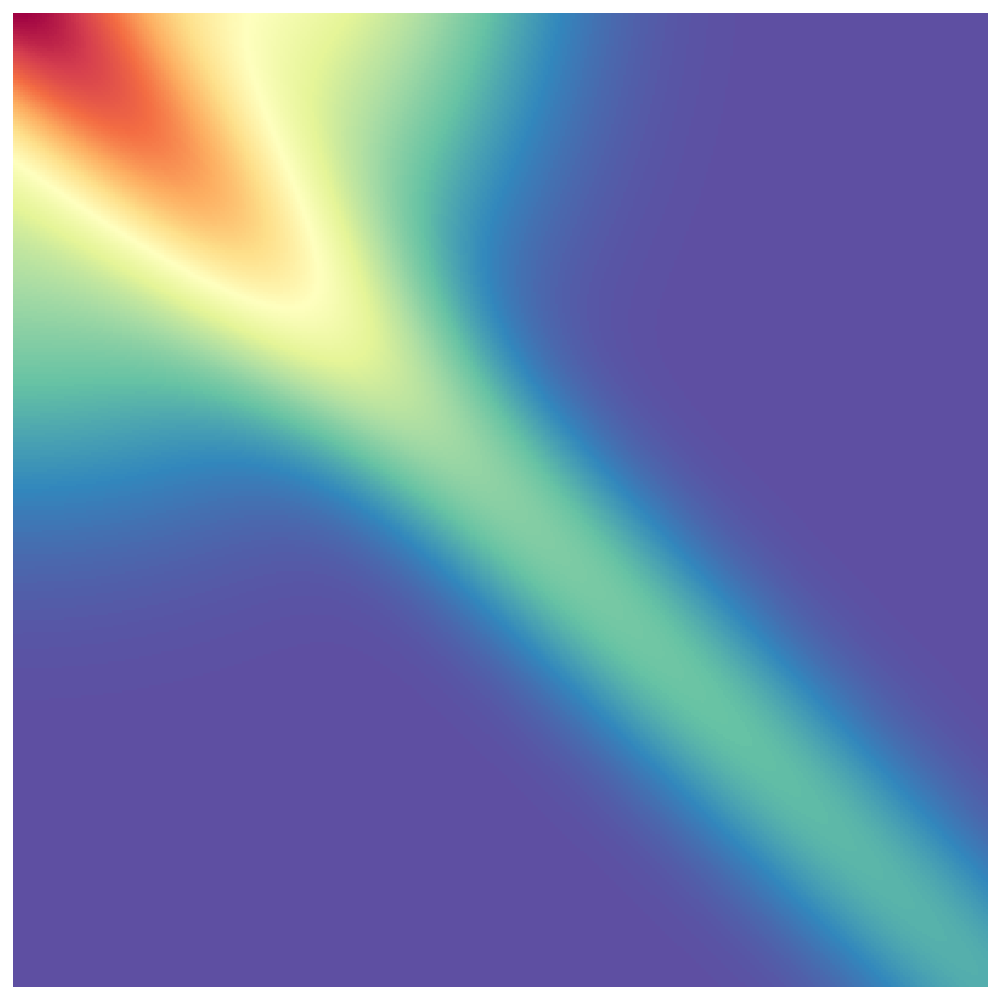
\includegraphics{highfidelity.png}}}
\end{bmatrix}
\!\!
\begin{bmatrix}
\vcenter{\hbox{
\includegraphics{basis.png}}}
\end{bmatrix}
\!\!
% \longrightarrow
=
\!\!
\begin{bmatrix}
\vcenter{\hbox{
\includegraphics{projected_matrix.png}}}
\end{bmatrix}

$

&

$

\begin{bmatrix}
\vcenter{\hbox{
\includegraphics{projected_matrix.png}}}
\end{bmatrix}
\!\!
\begin{bmatrix}
\vcenter{\hbox{
\includegraphics{coefficients.png}}}
\end{bmatrix}
\!\!
=
\widetilde E
\begin{bmatrix}
\vcenter{\hbox{
\includegraphics{coefficients.png}}}
\end{bmatrix}
\!\!
$\\

\!\!\!$N_h \times N_h$\hspace{0.75in} & $N_h \times n_b$ & \hspace{0.2in}$n_b \times N_h$\hspace{0.55in}$N_h \times N_h$\hspace{0.3in}$N_h \times n_b$\hspace{0.25in}$n_b \times n_b$ &
% $n_b \times n_b$\hspace{0.6in}
All size-$n_b$ operations

\\\midrule

% Time
% $t$
% &
Time:~
$\vcenter{\hbox{
\includegraphics{time_long.png}}}$ per $\theta$ sample &

\!\!\!$n_b \times \vcenter{\hbox{
\includegraphics{time_long.png}}}$\!\!\!

&

$\sim \vcenter{\hbox{
\includegraphics{time_long.png}}}$

&

\!\!\!\!%
Sampling $\theta$: $\vcenter{\hbox{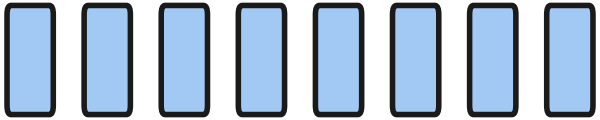
\includegraphics{time_short.png}}}$
\!\!\!\!%
\\

\bottomrule
\end{tabular}

\end{document}
